\documentclass{article}

\usepackage[final]{neurips_2019}
% numeric citation style ([1], [2], ...) instead of author-year
\setcitestyle{numbers,square,comma}

\usepackage[utf8]{inputenc}
\usepackage[T1]{fontenc}
\usepackage{hyperref}
\usepackage{url}
\usepackage{booktabs}
\usepackage{multirow}
\usepackage{amsfonts}
\usepackage{amsmath}
\usepackage{amssymb}
\usepackage{nicefrac}
\usepackage{microtype}
\usepackage{graphicx}
\usepackage{xcolor}
\usepackage{lipsum}

\newcommand{\note}[1]{\textcolor{blue}{[{#1}]}}

% two-value cell: gray = accuracy on ground-truth label, black = targeted attack success rate
\newcommand{\cell}[2]{{\color{gray}#1}\,/\,#2}
% clean cell: only ground-truth accuracy (gray)
\newcommand{\ccell}[1]{{\color{gray}#1}}

% prompt-mode illustration: highlight colors
\definecolor{hlQ}{HTML}{D6E4F0} % question / prompt
\definecolor{hlP}{HTML}{FCE5CD} % answer priming
\definecolor{hlT}{HTML}{D9EAD3} % teacher-forced candidate
\definecolor{hlA}{HTML}{E6D9F0} % assistant role tag
\definecolor{barcol}{HTML}{3D6FB4} % logit bar
\newcommand{\hlQ}[1]{\colorbox{hlQ}{#1}}
\newcommand{\hlP}[1]{\colorbox{hlP}{#1}}
\newcommand{\hlT}[1]{\colorbox{hlT}{#1}}
\newcommand{\hlA}[1]{\colorbox{hlA}{#1}}
% horizontal logit bar of given length (in pt)
\newcommand{\logit}[1]{\textcolor{barcol}{\rule[-0.4ex]{#1pt}{1.6ex}}}

\title{
  Adversarial Examples on Visual Language Models \\
  \vspace{1em}
  \small{\normalfont RUB Responsible AI Course Project}
}

\author{
  Yingte Xu\\
  Ruhr University Bochum \\
  \texttt{yingte.xu@edu.ruhr-uni-bochum.de}
}

\begin{document}

\maketitle

\begin{abstract}
The study of adversarial examples shows the vulnerability of image classifiers and visual encoders. 
With the development of language models with visual modalities (VLMs), it is important to check whether they inherit the vulnerability of encoders, and to what extend the adversarial examples will transfer among different VLMs.
Our experiments are based on CLIP336 (the visual encoder), LLaVA and VisualRWKV (two VLMs using CLIP336). We train and evaluate adversarial examples for image classification from the Imagenette dataset.
Our result shows that adversarial examples trained on visual encoders are more transferable, and an end-to-end adversarial training will overfit on the langauge model and target prompt.
\end{abstract}


% {\color{red} This template does not contain the full instruction set for this assignment; please refer back to the milestone instructions PDF.}

\section{Introduction}

Machine learning models now have the human-level capabilities in many tasks, including image classification, audio understanding and text generation. 
But models follow a totally different mechanism than human, and they have unique vulnerabilities.
Adversarial example is such a case.
It refers to the scenario that attackers can construct input examples that steer and change the output in an unexpected way.
One typical type of adversarial examples happens in image classification.
In 2015, Goodfellow et al.~\cite{Goodfellow2015FGSM} demonstrated a constructed adversarial example that deceives the image classifier GoogLeNet~\cite{Szegedy2015GoogLeNet}. 
The clean image is correctly classified as a panda with 57.7\% confidence. But with a small perturbation of magnitude $\epsilon = 0.007$, the adversarial example is misclassified as a gibbon with 99.3\% confidence.
The adversarial examples are not distinguishable with clean ones to human eyes, and this discovery reveals a type of real and critical vulnerability that can be utilized maliciously.



Adversarial example follows the form of a white-box attack.
The attacker has knowledge of the entire inference structure and weight of the model. The adversarial example is fabricated by minimizing the cross-entropy loss on the target label, and performing gradient decent on the input example rather than model weight.
The common explanation for the existence of adversarial labels is the large input space.
For images with 8 bit-depth and 3 channels, the total count of all possible variants goes to $256^{3\times W \times H}$, where $W$ and $H$ denote weight and height in pixel number.
All the images form a high-dimensional space, and different image categories correspond to different low-dimensional manifolds~\cite{Fefferman2016Manifold}.
Therfore, it is easy to find approximate but out-of-distribution samples that the model has never seen, and adversarial examples exploit this fact.


With the surge of LLM in recent years, it would be meaningful to ask whether similar attacks can be performed on language models, especially those with multiple modalities besides text.
The design of multimodal language models usually consists of one pretrained language model backbone, and the encoders that embed multimodal input as tokens in the LM semantic space. Therefore, it would be likely that multimodal langauge models inherit the vulnerability of encoders as well. And since language models process and generate text, there are even more aspects exposed to adversarial example attacks other than simple classification. 
For example, an attacker may be able to bypass the safeguard or retrieve sensitive information with an adversarial image input.
Another concern is the transferability of adversarial examples.
Since different models may share the same encoder, we want to understand how generic the adversarial examples are.

This work focuses on Visual Language Models based on the CLIP336 visual encoder, and studies the construction and transferability of adversarial examples. 
In particular, we choose two VLMs that use CLIP336 as the visual encoder: LLaVA-1.5 7B~\cite{Liu2024LLaVA15} and VisualRWKV-6 7B~\cite{Hou2025VisualRWKV}.
We investigate attacks on image classification and jailbreaks.
Our results show that these VLMs are vulnerable to adversarial image attacks, and the examples are transferable in general. 
In classification, we find that adversarial examples trained only on the visual encoder work in more general cases than those trained end-to-end on LLaVA. 

These discoveries suggest that the vulnerability does come from the encoder, and the end-to-end training of adversarial examples will overfit on the language model backbone.







\section{Related Work}

The first adversarial example attack was ...

... studies the transferability of adversarial examples.


Multimodal language models incorporates rich modalities like vision and audio into the language model backbone. Representative examples include open-source models ... and closed-source models ....

... first applies adversarial examples to VLM.

There is also research on adversarial examples on language models with acoustic modalities ... 



Schaeffer et al.~\cite{Schaeffer2025} conducted an experiment on over 40 open-source VLM, and claims that end-to-end jailbreak attacks do not transfer in general, even with matching visual encoders or language models.


About defense,

... proposed the defense by by training on adversarial examples and improve the robustness.

Robust CLIP~\cite{Robust-CLIP} verified that roubstness training for image classification on the visual encoders can generalize to VLMs in a plug-in way.
%
Yin et al.~\cite{Yin_2026_CVPR} point out that encoder-only robustnes training is not sufficient against jailbreak attacks. An end-to-end training incorporating all modalities works better.

\note{We need a graph from raw image to resized, image01, pixel-values.}

\begin{figure}[t]
  \centering
  \setlength{\tabcolsep}{3pt}
  \begin{tabular}{@{}c@{\hspace{0.5em}}cccc@{}}
    \rotatebox[origin=c]{90}{\footnotesize clean} &
    \raisebox{-0.5\height}{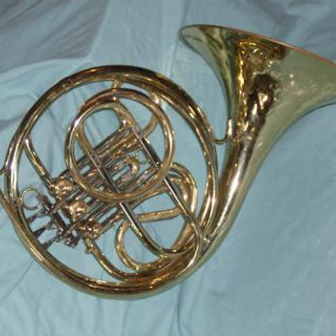
\includegraphics[width=0.21\textwidth]{figures/sample0_orig.png}} &
    \raisebox{-0.5\height}{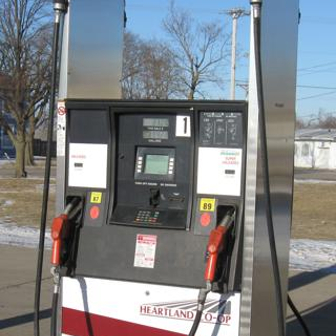
\includegraphics[width=0.21\textwidth]{figures/sample1_orig.png}} &
    \raisebox{-0.5\height}{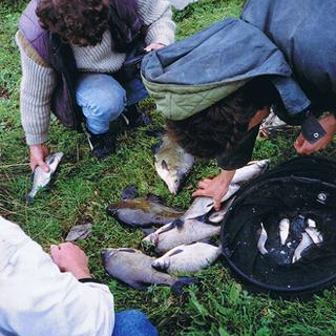
\includegraphics[width=0.21\textwidth]{figures/sample2_orig.png}} &
    \raisebox{-0.5\height}{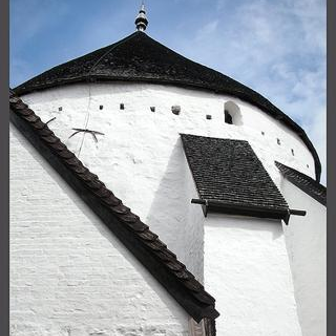
\includegraphics[width=0.21\textwidth]{figures/sample3_orig.png}} \\[2pt]
    \rotatebox[origin=c]{90}{\footnotesize adversarial} &
    \raisebox{-0.5\height}{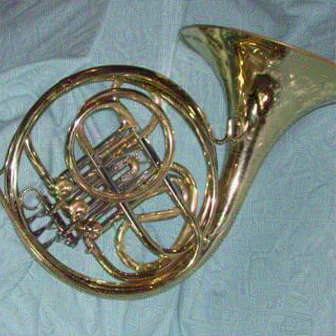
\includegraphics[width=0.21\textwidth]{figures/sample0_adv.png}} &
    \raisebox{-0.5\height}{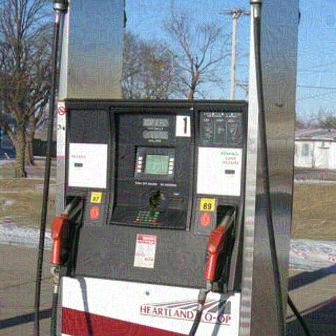
\includegraphics[width=0.21\textwidth]{figures/sample1_adv.png}} &
    \raisebox{-0.5\height}{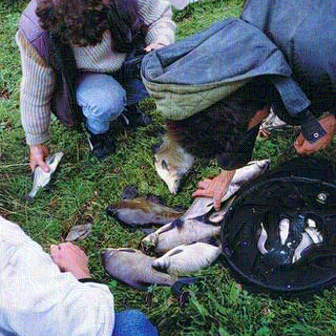
\includegraphics[width=0.21\textwidth]{figures/sample2_adv.png}} &
    \raisebox{-0.5\height}{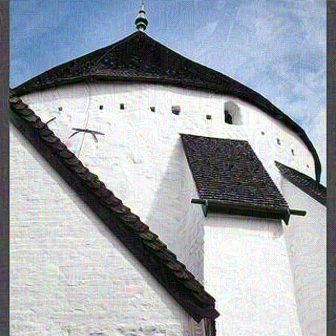
\includegraphics[width=0.21\textwidth]{figures/sample3_adv.png}} \\[4pt]
    &
    \scriptsize\shortstack{French horn $\to$ gas pump\\ $\mathrm{MSE} = 3.49\times10^{-4}$} &
    \scriptsize\shortstack{gas pump $\to$ golf ball\\ $\mathrm{MSE} = 3.11\times10^{-4}$} &
    \scriptsize\shortstack{tench $\to$ French horn\\ $\mathrm{MSE} = 3.17\times10^{-4}$} &
    \scriptsize\shortstack{church $\to$ cassette player\\ $\mathrm{MSE} = 2.87\times10^{-4}$} \\
  \end{tabular}
  \caption{
    Samples from our adversarial Imagenette dataset.
    Top row: clean images (resized to $336\times336$); bottom row: the corresponding adversarial examples trained on the CLIP-336 encoder (resized space).
    Below each column: the ground-truth label, the attack target label, and the mean squared error (MSE) of the perturbation $\delta$ over all pixels in $[0,1]^{3\times336\times336}$ space, i.e.\ the same distance penalized during the attack (per-pixel $\ell_\infty \approx 0.06$).
    The perturbations are barely perceptible, yet each adversarial image is classified by CLIP as its target label.
  }
  \label{fig:dataset}
\end{figure}


\begin{table}[t]
  \centering
  \caption{
    Cross-evaluation of adversarial examples on Imagenette (accuracy in \%).
  }
  \label{tab:xeval}
  \vspace{0.5em}
  \small
  \begin{tabular}{@{}ll|cccccc@{}}
    \toprule
    \multirow{2}{*}{Model} & \multirow{2}{*}{Prompt} & \multirow{2}{*}{\shortstack{Clean\\(1024)}} & \multirow{2}{*}{Noise} & \multicolumn{2}{c}{CLIP-Adv (1024)} & \multicolumn{2}{c}{LLaVA-Adv (128)} \\
    \cmidrule(lr){5-6} \cmidrule(lr){7-8}
    & & & & image01 & resized & image01 & resized \\
    \midrule
    CLIP & --- & \ccell{99.5} & --- & \cell{2.4}{97.6} & \cell{2.2}{97.8} & \cell{78.9}{14.8} & \cell{78.1}{13.3} \\
    \midrule
    \multirow{3}{*}{LLaVA}
      & A & \ccell{97.0} & --- & \cell{62.1}{28.2} & \cell{60.9}{28.9} & \cell{7.8}{83.6} & \cell{8.6}{84.4} \\
      & B & \ccell{73.8}  & --- & \cell{46.3}{25.8} & \cell{45.8}{26.8} & \cell{39.8}{17.2} & \cell{42.2}{19.5} \\
      & C & \ccell{70.4}  & --- & \cell{50.3}{25.3} & \cell{49.9}{25.1} & \cell{46.9}{15.6} & \cell{50.0}{14.1} \\
    \midrule
    \multirow{3}{*}{VisualRWKV}
      & A & \ccell{96.8}  & --- & \cell{49.6}{47.9} & \cell{47.9}{49.3} & \cell{60.9}{21.9} & \cell{58.6}{20.3} \\
      & B & \ccell{93.1}  & --- & \cell{45.6}{45.3} & \cell{45.6}{44.9} & \cell{60.9}{19.5} & \cell{63.3}{17.2} \\
      & C & \ccell{94.2}  & --- & \cell{49.3}{40.4} & \cell{45.0}{44.0} & \cell{60.9}{12.5} & \cell{60.9}{12.5} \\
    \bottomrule
  \end{tabular}
\end{table}

\begin{table}[t]
  \centering
  \caption{
    The three prompt modes, shown as the \texttt{USER}/\texttt{ASSISTANT} conversation fed to the VLM.
    Highlights: \hlQ{prompt (question)}, \hlP{answer priming}, and \hlT{candidate label scored by teacher forcing}.
    For each image every class label is placed in the candidate slot; we score it by its log-likelihood under teacher forcing and predict the arg-max (\emph{``tench''} shown as an example).
    Mode A's option list is truncated here.
  }
  \label{tab:prompts}
  \vspace{0.5em}
  \footnotesize
  \begin{tabular}{@{}c l@{}}
    \toprule
    Mode & Conversation \\
    \midrule
    \multirow{2}{*}{A}
      & \ttfamily USER: <image> \hlQ{What is the main object in this photo? Options: tench, \dots} \\[2pt]
      & \ttfamily ASSISTANT: \hlP{The main object in this photo:}\hlT{ tench} \\
    \midrule
    \multirow{2}{*}{B}
      & \ttfamily USER: <image> \hlQ{What is the main object in this photo?} \\[2pt]
      & \ttfamily ASSISTANT: \hlP{The main object in this photo:}\hlT{ tench} \\
    \midrule
    \multirow{2}{*}{C}
      & \ttfamily USER: <image> \hlQ{What can you see in the photo?} \\[2pt]
      & \ttfamily ASSISTANT: \hlP{I can see a}\hlT{ tench} \\
    \bottomrule
  \end{tabular}
\end{table}

\begin{figure}[t]
  \centering
  $\begin{array}{r@{\hspace{1em}}l}
    & \hspace{0.7em}\text{\footnotesize candidate}\hspace{5em}\text{\footnotesize logits} \\[1pt]
    \text{\ttfamily ASSISTANT:}~\text{\hlP{The main object in this photo:}} &
    \left\{\begin{array}{@{}l@{\hspace{1.5em}}l@{}}
      \text{\hlT{tench}}            & \logit{15} \\[2pt]
      \text{\hlT{church}}           & \logit{32}~\Rightarrow\,\text{\footnotesize prediction} \\[2pt]
      \text{\hlT{English springer}} & \logit{22} \\[1pt]
      \multicolumn{1}{c}{\vdots}    & \\[1pt]
      \text{\hlT{parachute}}        & \logit{6} \\
    \end{array}\right.
  \end{array}$
  \caption{
    Teacher-forcing classification. After the \texttt{ASSISTANT} tag and the fixed \hlP{answer priming}, every class label is placed in the \hlT{candidate} slot in turn.
    Each candidate is teacher-forced and scored by the model's log-likelihood (its logits, drawn as bars).
    The candidate with the largest score (here \emph{church}) is taken as the classification result.
  }
  \label{fig:teacherforcing}
\end{figure}


\section{Conclusion}

End-to-end attack on VLM will overfit on the language model and damage transferability.

\bibliographystyle{unsrtnat}
\bibliography{references}

\end{document}
